\documentclass[10pt, compress, onlymath]{beamer}
\usefonttheme{serif}
\usetheme[nooffset]{m}

\usepackage{booktabs}
\usepackage[scale=2]{ccicons}
\usepackage{minted}
\usepackage{graphicx}

%\newcommand{\lmr}{\fontfamily{lmr}\selectfont} % Latin Modern Roman
%\renewcommand\rmdefault{lmr}
%\renewcommand\sfdefault{lmss}
%\renewcommand\ttdefault{lmtt}

\usepgfplotslibrary{dateplot}

\usemintedstyle{trac}

\title{Crowdsourcing}
\subtitle{}
\date{May 5, 2015}
\author{Stephen Mayhew, Daniel Khashabi}
\institute{University of Illinois at Urbana Champaign}

\begin{document}

\maketitle

\begin{frame}[fragile]
  \frametitle{Baselines}
  \begin{enumerate}
  \item Majority Voting
  \item Hubs and Authorities
  \item Singular vector approach
  \item EM
  \item \textbf<2>{EM with priors}
  \item \textbf<2>{Iterative Weighted Majority Voting}
  \item Simplified BP
  \item \textbf<2>{Discretized BP}
  \item Tree-reweighted message passing\footnote{never finished...}
  \item Spectral Meets EM$^1$
  \end{enumerate}


\end{frame}


\begin{frame}[fragile]
  \frametitle{EM with Priors}
Define
\[g_{ij}(t_i, p_j) = p_j \mathbf{I} \left\lbrace  A_{ij}=  t_i  \right\rbrace +  (1-p_j ) \mathbf{I} \left\lbrace  A_{ij} \neq  t_i  \right\rbrace\]


\pause
Full likelihood (with Beta priors):

\[ \mathcal{L}(p; t) = \prod_{i,j} g_{ij}(t_i,p_j) \prod_j \left( c+ \frac{1-c}{B(\alpha, \beta)} p_j^{\alpha-1} (1-p_j)^{\beta-1}  \right) \]
\pause

M-Step becomes:
\[
p_j = \frac{ \alpha - 1 + \sum_jq(A_{ij}) }{ \alpha + \beta-2 + \sum_jq(A_{ij})  + \sum_j q(-A_{ij})  }
\]

(Note: this same result is a lower bound on the situation where priors come from $p_j = 0.1 + 0.9Z$)

\end{frame}

\begin{frame}[fragile]
  \frametitle{Iterative Weighted Majority Voting (IWMV)}

From \textit{Error Rate Bounds and Iterative Weighted Majority Voting
for Crowdsourcing} by Hongwei Li and Bin Yu\footnote{\texttt{http://arxiv.org/pdf/1411.4086v1.pdf}}

\centering
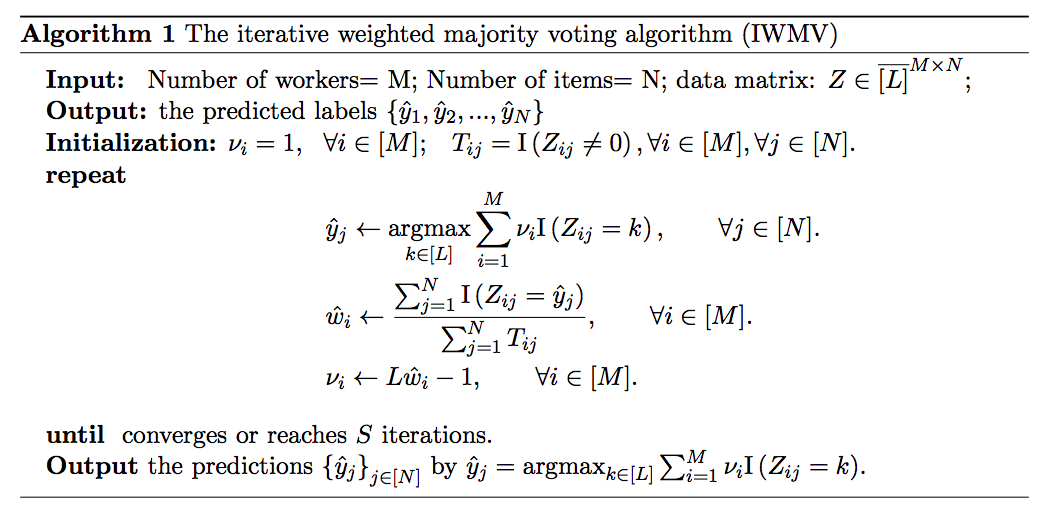
\includegraphics[scale=0.30]{iwmv.png}

\end{frame}

\begin{frame}[fragile]
  \frametitle{Discretized BP}

Original BP udpates are:
\begin{align*}
y^{(k)}_{a \to i}(p_a) &\propto \mathcal{F}(p_a) \prod_{j \in \partial a \backslash i} \left\{(p_a + \bar{p}_a + (p_a - \bar{p}_a)A_{ja})x_{j\to a}^{(k)}(+1) + (p_a + \bar{p}_a - (p_a - \bar{p}_a)A_{ja})x_{j\to a}^{(k)}(-1)  \right\}\\
x^{(k+1)}_{i \to a}(\hat{t}_i) &\propto \prod_{b \in \partial i\backslash a} \int \Big(y_{b \to i}^{(k)}(p_b)(p_b \mathbb{I}_{(A_{ib}=\hat{t}_i)} + \bar{p}_b \mathbb{I}_{(A_{ib}\neq\hat{t}_i)})\Big)dp_b
\end{align*}

\pause

Discretize $p_j$:
\begin{align*}
x^{(k+1)}_{i \to a}(\hat{t}_i) &\propto \prod_{b \in \partial i\backslash a} \sum_{p_b \in P} \Big(y_{b \to i}^{(k)}(p_b)(p_b \mathbb{I}_{(A_{ib}=\hat{t}_i)} + \bar{p}_b \mathbb{I}_{(A_{ib}\neq\hat{t}_i)})\Big)
\end{align*}

For $P = \{ p_1, p_2, p_3, ..., p_k\}$

\end{frame}


\begin{frame}[fragile]
  \frametitle{Graph}

\centering
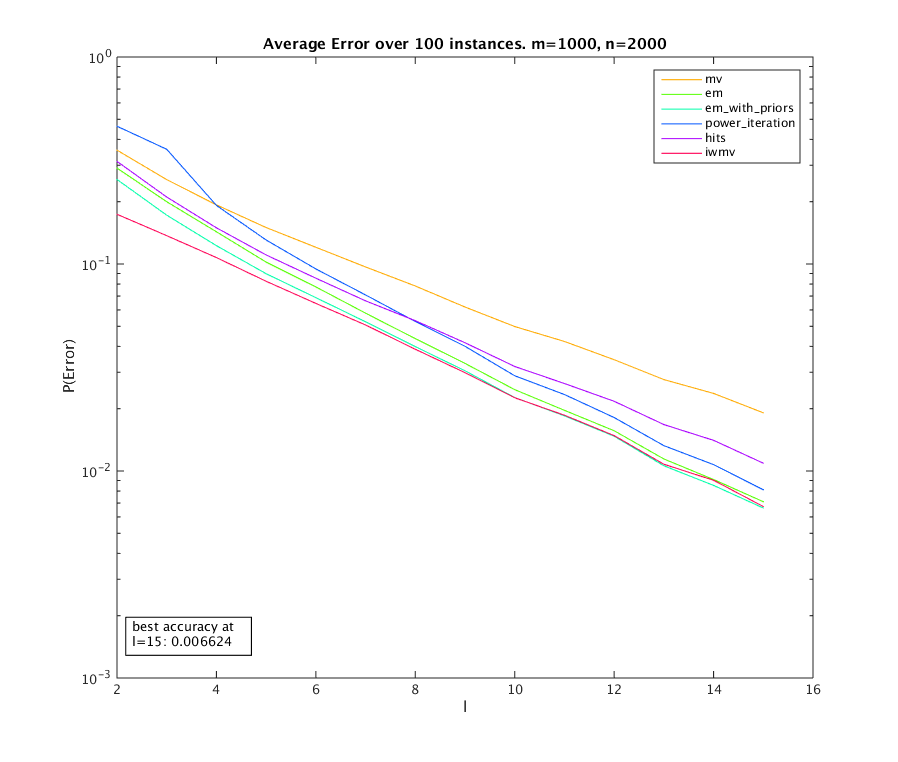
\includegraphics[scale=0.4]{all.png}


\end{frame}

\begin{frame}[fragile]
  \frametitle{Graph}

\centering
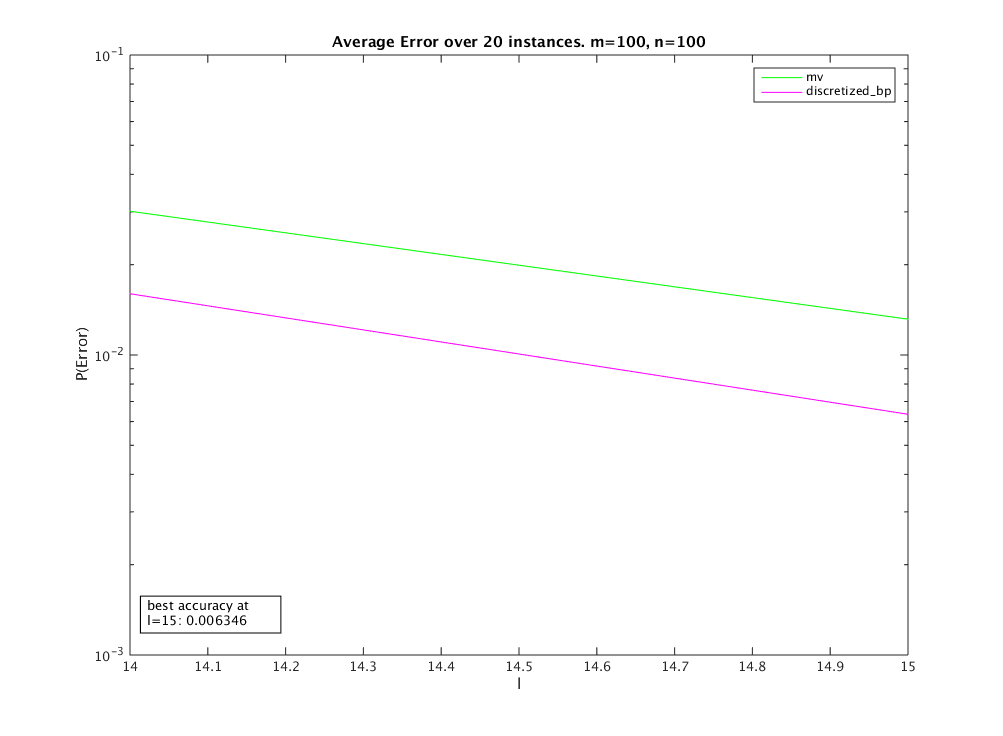
\includegraphics[scale=0.4]{mv_discretized.png}


\end{frame}

\begin{frame}[fragile]
  \frametitle{Table}

\begin{table}[htdp]

\begin{center}
\begin{tabular}{|c|c|l|}
\hline
Algorithm & $m,n$ & $\ell = 15$ \\
\hline
Discretized BP & 100,100 & 0.006346 \\
EM with Priors & 100,100 & 0.008478 \\
EM with Priors & 1000,2000 & 0.006624 \\
EM with Priors & 250,2000 & 0.005512 \\
Simplified BP & 250,2000 & 0.005466 \\
IWMV & 250,2000 & 0.0057\\
\hline
\end{tabular}
\end{center}
\label{default}
\end{table}%



\end{frame}


%\plain{Questions?}

\end{document}
